% XeLaTeX can use any Mac OS X font. See the setromanfont command below.
% Input to XeLaTeX is full Unicode, so Unicode characters can be typed directly into the source.

% The next lines tell TeXShop to typeset with xelatex, and to open and save the source with Unicode encoding.

%!TEX TS-program = xelatex
%!TEX encoding = UTF-8 Unicode

\documentclass[11pt]{article}
\usepackage{geometry}                % See geometry.pdf to learn the layout options. There are lots.
\geometry{a4paper}                   % ... or a4paper or a5paper or ... 
%\geometry{landscape}                % Activate for for rotated page geometry
%\usepackage[parfill]{parskip}    % Activate to begin paragraphs with an empty line rather than an indent
\usepackage{graphicx}
\usepackage{amssymb}

\usepackage{url}
\usepackage{verbatim}
\usepackage{color}

\definecolor{listing_background_color}{rgb}{0.9,0.85,0.8}
\definecolor{darkgreen}{rgb}{0,0.4,0}

\usepackage{listings}
\lstdefinelanguage{JavaScript}{
  keywords={typeof, new, true, false, catch, function, return, null, catch, switch, var, if, in, while, do, else, case, break},
  keywordstyle=\color{blue}\bfseries,
  ndkeywords={class, export, boolean, throw, implements, import, this},
  ndkeywordstyle=\color{darkgray}\bfseries,
  identifierstyle=\color{black},
  sensitive=false,
  comment=[l]{//},
  morecomment=[s]{/*}{*/},
  commentstyle=\color{darkgreen}\ttfamily,
  stringstyle=\color{red}\ttfamily,
  morestring=[b]',
  morestring=[b]"
}
\lstset{ %
language=HTML,                % choose the language of the code
basicstyle=\footnotesize,       % the size of the fonts that are used for the code
%numbers=left,                   % where to put the line-numbers
%numberstyle=\footnotesize,      % the size of the fonts that are used for the line-numbers
%stepnumber=2,                   % the step between two line-numbers. If it's 1 each line 
                                % will be numbered
%numbersep=5pt,                  % how far the line-numbers are from the code
backgroundcolor=\color{listing_background_color},  % choose the background color. You must add \usepackage{color}
showspaces=false,               % show spaces adding particular underscores
showstringspaces=false,         % underline spaces within strings
showtabs=false,                 % show tabs within strings adding particular underscores
frame=single,	                % adds a frame around the code
tabsize=2,	                % sets default tabsize to 2 spaces
captionpos=b,                   % sets the caption-position to bottom
breaklines=true,                % sets automatic line breaking
breakatwhitespace=false,        % sets if automatic breaks should only happen at whitespace
title=\lstname,                 % show the filename of files included with \lstinputlisting;
                                % also try caption instead of title
escapeinside={\%*}{*)},         % if you want to add a comment within your code
morekeywords={*,...}            % if you want to add more keywords to the set
}





% Will Robertson's fontspec.sty can be used to simplify font choices.
% To experiment, open /Applications/Font Book to examine the fonts provided on Mac OS X,
% and change "Hoefler Text" to any of these choices.

\usepackage{fontspec,xltxtra,xunicode}
\defaultfontfeatures{Mapping=tex-text}
\setromanfont[Mapping=tex-text]{Georgia}
\setsansfont[Scale=MatchLowercase,Mapping=tex-text]{Gill Sans}
\setmonofont[Scale=MatchLowercase]{Monaco}




\definecolor{CodeColor}{rgb}{0.8,0.8,0.8}
\makeatletter\newenvironment{codebox}{%
   \begin{lrbox}{\@tempboxa}\begin{minipage}{\columnwidth}}{\end{minipage}\end{lrbox}%
   \colorbox{CodeColor}{\usebox{\@tempboxa}}
}\makeatother




\title{Getting started with i2maps}
\author{Christian Kaiser}
\date{}                     % Activate to display a given date or no date

\begin{document}
\maketitle


This guide goes through the process of downloading and installing i2maps on a desktop computer, and how to create a simple project. The purpose is to get you started with the most common aspects of i2maps.



\section{Installation}

\subsection{Requirements}

\begin{itemize}
\item One of the following operating systems:
	\begin{itemize}
		\item Linux (tested with Ubuntu 9.04, 9.10, 10.04, 10.10)
		\item Mac OS X (tested with OS X 10.6)
	\end{itemize}
	Other operating systems might work also, but have not been tested.

\item Python version 2.6 or later.
\item Python setuptools
\item \verb=GEOS, GDAL, PROJ.4= and \verb=SQLite= libraries
\item The following Python modules are mandatory for running i2maps: \texttt{django, geos, gdal, numpy, sqlite}
\item For some functions, PostGIS is strongly recommended.
\item In order to have the full functionality, the following Python modules are needed additionally: \texttt{psycopg2, geojson, shapely}
\end{itemize}


\subsection{Installation on Ubuntu}

\begin{enumerate}

	\item Install the following libraries and modules with all dependencies directly using the APT system: \texttt{python-django, libgdal1-1.6.0, gdal-bin, libgeos-3.2.0, libproj0, libsqlite3-0, python-numpy, python-setuptools}

	\item Install the django Python package using the setuptools: \\
	\texttt{sudo easy\_install django}

	\item Download the i2maps package from \url{http://ncg.nuim.ie/i2maps/} and extract the archive.

	\item Copy the i2maps folder into the site-packages folder of your Python installation (typically \texttt{/usr/local/lib/python2.6/dist-packages}). You probably need to do this with administrator rights (as \texttt{sudo}).

	\item Copy the \verb=i2maps_working_dir= folder from the i2maps archive to a convenient location (e.g. in your home folder).

	\item Start the i2maps development server using the following commands. Put the correct path to your i2maps package (on the first line) and i2maps working directory (on the second line). Don't forget the trailing '/' on the second line! \\
	\texttt{cd /usr/local/lib/python2.6/dist-packages/i2maps \\
	export i2maps\_working\_directory=/path/to/your/i2maps\_working\_dir/ \\
	python i2maps\_server.py}
	
	You should have the following output: \\
	\texttt{i2maps development server is running at http://127.0.0.1:8000/ \\
	i2maps working directory: /home/christian/i2maps\_working\_dir/ \\
	Quit the server with CONTROL-C.}
	
	If yes, everything went fine. Leave the window open until you don't need the i2maps server anymore. Go to your favourite browser (we recommend Google Chrome), and go to \url{http://127.0.0.1:8000/} and then \url{http://127.0.0.1:8000/projects/example1/index.html}.
	
\end{enumerate}


	
\subsection{Installation on Mac OS X (Snow Leopard)}

\begin{enumerate}
	\item Install the following frameworks from \url{http://www.kyngchaos.com}: \texttt{UnixImageIO, PROJ, GEOS, SQLite3, GDAL}. There might be a convenience installer \verb=GDAL Complete= installing at once all the mentioned frameworks.
	
	\item Download the i2maps package from \url{http://ncg.nuim.ie/i2maps/}
\end{enumerate}





\section{The i2maps working directory}

i2maps is composed by a Python package, and a working directory. This working directory contains all files and data needed for the different projects. We have already prepared a working directory containing an example project. You might want to download the example working directory from \url{http://ncg.nuim.ie/i2maps/docs/uploads/i2maps_working_dir.zip}.
Extract the ZIP file to a convenient location, for example in your home folder. The working directory, named \verb=i2maps_working_dir= by default, contains three subfolders: \texttt{datasources, processors,} and \texttt{views}.

The folder datasources contains everything that is needed for retrieving the data for a given project. This can be a SQLite database, the connection settings for a PostGIS database, and Python code that can be called for getting and/or setting the data in some specified way.
The folder processors contains code that is used to run data crawlers, models and other tasks that are usually done in the background, for example at a given time.

The folder views finally contains one folder for each i2maps project, where are stored all the files publicly accessible over the Web. Usually, these are the HTML and JavaScript files for the project. However, don't put any Python code in this folder, as it can be directly downloaded from the Web.






\section{Setting up our first i2maps project (example 1)}

This is a step-by-step tutorial how to set up a simple i2maps project. Basically, it will work through the example provided when downloading i2maps.

This example project is a simple interactive map of Ireland, where we have a couple of base layers (e.g. OpenLayers and Google Maps), together with around 25 temperature sensors at a fixed location depicted as coloured circles on the map, and an interpolated (predicted) surface showing the temperature at each location in Ireland as a raster layer. It is possible for the user to query the predicted temperature with the mouse; the temperature at the current mouse position is shown in a legend, and when clicking with the mouse at a location on the surface, a new circle is inserted and some additional information displayed. The prediction of the temperature uses as input data the temperature sensors and the digital elevation model for Ireland. The method used for calculating is a Kernel regression. Figure~\ref{fig:ex1_layout} shows the layout of the project.

\begin{figure}
	\begin{center}
	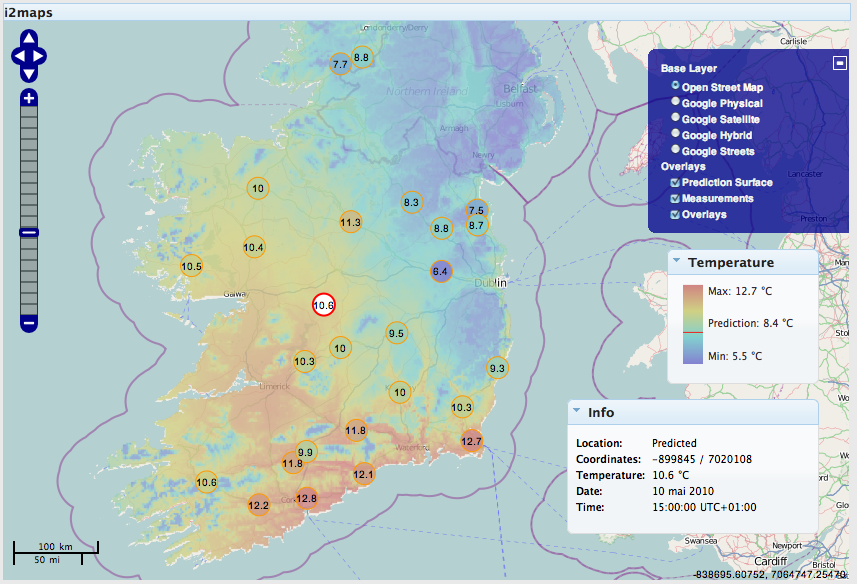
\includegraphics[width=12cm]{figures/ex1_layout.png}
	\caption{The first i2maps project in the browser}
	\label{fig:ex1_layout}
	\end{center}
\end{figure}

For setting up the project, we will divide the work in the following parts:

\begin{enumerate}
	\item Preparing the base data for the project. This implies gathering the information about the temperature sensors and the measurements.
	\item Setting up the project layout. This means preparing the HTML file underlying the project.
	\item Preparing the JavaScript for loading the base layers and display the layer containing the temperature sensors.
	\item Prepare the interface for delivering the temperature sensor data from the database (prepared in step 1) to the i2maps client (to the JavaScript). This involves setting up the i2maps data source for our project.
	\item Writing a processor script for computing the predicted temperature surface.
	\item Adapting the JavaScript and the i2maps data source for displaying the temperature surface in the browser.
\end{enumerate}

After these steps, you will (hopefully) understand the base structure of i2maps and be able to use the software in a similar project with your own data.


\subsection{Prepare the database}

Our base data contain information about the temperature sensors (id, name, location, elevation) and about the temperature measurements taken by these sensors (time and temperature). In our first example, we will consider the temperature measurements for only one moment in time. We are going to store the data in a SQLite database containing two tables: sensors and measurements. Figure~\ref{fig:ex1_dbstructure} shows the database structure. The database is already included in the i2maps example working directory, in \texttt{datasources/example1/example1.db}. You can use a graphical user interface to SQLite to explore the database, e.g. SQLite Database Browser available at \url{http://sqlitebrowser.sourceforge.net} (on Ubuntu install by typing \texttt{sudo apt-get install sqlitebrowser}) or Sqliteman available at \url{http://sqliteman.com} (on Ubuntu type \texttt{sudo apt-get install sqliteman}). These tools also help you loading the data from a CSV file into the database.

\begin{figure}
	\begin{center}
	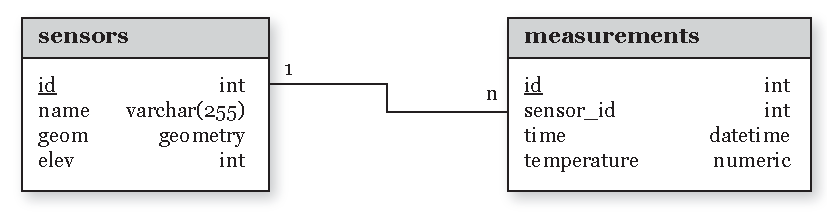
\includegraphics[]{figures/ex1_dbstructure.pdf}
	\caption{The structure of our SQLite database}
	\label{fig:ex1_dbstructure}
	\end{center}
\end{figure}

Once the database prepared, store it in your i2maps working directory, in the folder \texttt{datasources/example1/example1.db}.



\subsection{Preparing the page layout}

Now we are ready for preparing the page layout of our project; this means setting up the HTML code. We will call this file \texttt{index.html} and it will go in the folder \texttt{views/example1} in your i2maps working directory.

This file is a usual HTML file that you can customise as you wish. In order to get the i2maps functionalities to work, we need to insert some specific code at a given place:

\begin{itemize}

\item Include the i2maps Javascript library in the header using the following code: \\
\texttt{<script type="text/javascript" src="../../media/js/i2maps.js"></script>}

\item Create a main i2maps container where all the i2maps content will go: \\
\texttt{<div id="i2maps\_tabl" class="panel ui-widget ui-panel"> \\
</div>} \\
We give the \texttt{DIV} container the ID ''i2maps\_tabl``. The container has 3 CSS classes. We don't need to care where these CSS styles are defined, they will be included automatically by the i2maps JavaScript library (in fact, the style sheets are located inside the i2maps package, in the folder \texttt{media/css}).

\item Inside our main i2maps container, we will need to insert some more content. We will first insert the title of our map: \\
\texttt{<h3 class="ui-widget ui-panel-header ui-widget-header" style="width: 98\%;">i2maps</h3>}

\item We will also include a placeholder container for displaying messages. Basically, i2maps will take any DIV it finds with ID ''message`` for displaying the different messages. This code goes also inside the main i2maps container: \\
\texttt{<div id="message" style="width: 98\%"></div>}

\item We include another container for the map area itself (of course). We will give this DIV the ID ''map\_canvas``. We will use this ID later in our project JavaScript to indicate the i2maps library where to draw the map. \\
\texttt{<div id="map\_canvas" style="width: 98\%; height: 95\%; position: relative; left:0px; top:0px;"></div>}

\item Finally, we can create any number of these floating ''Info`` or ''Legend`` boxes. We do this by creating another DIV that we include inside the main i2maps container. We can include some information on where to place the container (inside the \texttt{style} property):
\begin{verbatim}<div id="legend_box" class="panel" style="position: fixed; 
right: 50px; bottom: 230px; height: 110px; width: 150px; 
margin-left: 5px;">
    <h3>Temperature</h3>
    <div>
        <div id="legend" style="overflow: auto; height: 90px; 
        padding-left: 10px;"></div>
    </div>
</div>
\end{verbatim}
Of course, we can include any HTML code inside the most nested container to display some initial information, as it is done with the info box.
\end{itemize}

The complete HTML, as provided in the i2maps example working directory, is as follows (everything between \verb=<!--= and \verb=-->= are comments). There is also a line for including our own project JavaScript file (\verb=script.js=).

\begin{lstlisting}
<html>
<head>
	<title>i2maps - Example 1 (weather)</title>
	<!-- Load the i2maps JavaScript library: -->
	<script type="text/javascript" src="../../media/js/i2maps.js"></script>
	<!-- Load our own project JavaScript file: -->
	<script type="text/javascript" src="script.js"></script>
</head>

<body style="background-color: #e9e9e9;">
	<!-- The main container for i2maps -->
	<div id="i2maps_tabl" class="panel ui-widget ui-panel" style="padding-top: 3px; padding-left: 3px">
		<!-- The i2maps heading -->
		<h3 class="ui-widget ui-panel-header ui-widget-header" style="width: 98%;">i2maps</h3>
		<div>
			<!-- An empty containing for displaying all messages coming from i2maps -->
			<div id="message" style="width: 98%"></div>
			
			<!-- The main div containing the map -->
			<div id="map_canvas" style="width: 98%; height: 95%; position: relative; left:0px; top:0px;"></div>
			
			<!-- The floating info box -->
			<div id="info_box" class="panel" style="position: fixed; right: 50px; bottom: 80px; height: 110px; width: 250px; margin-left: 5px;">
				<h3>Info</h3>
				<div>
					<div id="attributes" style="overflow: auto; height: 90px;">
						<p style="font-size: 10px; margin: 5px; margin-top: 0px; margin-bottom: 0px;">Click on one of the points to retrieve additional information on a measurement.</p>
						<p style="font-size: 10px; margin: 5px; margin-top: 0px; margin-bottom: 0px;">Click on the temperature surface to see additional information about the predicted temperature.</p>
					</div>
				</div>
			</div>
			
			<!-- The legend box -->
			<div id="legend_box" class="panel" style="position: fixed; right: 50px; bottom: 230px; height: 110px; width: 150px; margin-left: 5px;">
				<h3>Temperature</h3>
				<div>
					<div id="legend" style="overflow: auto; height: 90px; padding-left: 10px;"></div>
				</div>
			</div>	
					
		</div>
	</div>
</body>
</html>
\end{lstlisting}




\subsection{Preparing the project JavaScript code}

In order to get our i2maps project to work, we need to write a JavaScript file that will automatically be called by the i2maps JavaScript library. It specifies all the parameters of our map and the additional controls around the map. This script is located at the same place as the \texttt{index.html} created in the previous step. The file \texttt{index.html} needs to have a line for including this script that is usually named just \texttt{script.js}: \\
\texttt{<script type="text/javascript" src="script.js"></script>}.

A minimal script looks like this:
\begin{lstlisting}[language=JavaScript]
i2maps.setupProject(function() {
	var map = new i2maps.Map({id: 'map', mapDiv: 'map_canvas'});
	i2maps.registerMap(map);
});
\end{lstlisting}

Basically, it is a call to the method \texttt{setupProject} of the global variable \texttt{i2maps}. The only argument of this method is a (potentially long) function that will be executed automatically by the i2maps JavaScript library. In its minimal shape, this function just creates a new i2maps map (with ID ''map`` and using the DIV with ID ''map\_canvas``), and registers this map with the global i2maps object.

In this section, we are now going to extend this small function to include more and more functionality.

In a first step, we are going to activate the ''Info`` and ''Legend`` boxes by telling i2maps that they are a ''panel``. We can execute this code at any stage of the function, but we choose to do so at the end for a better readability:

\begin{lstlisting}[language=JavaScript]
i2maps.setupProject(function() {
	var map = new i2maps.Map({id: 'map', mapDiv: 'map_canvas'});
	i2maps.registerMap(map);
	
	// Activate the Info Box and legend Panels
	$("#info_box").panel({
		draggable: true, collapsible: true, collapsed: false
	});
	$("#legend_box").panel({
		draggable: true, collapsible: true, collapsed: false
	});
});
\end{lstlisting}

Now, we are going to insert a vector layer with the location of the temperature sensors and the values of the measurements. i2maps is using OpenLayers (\url{http://www.openlayers.org}) as mapping engine. Each layer that we are going to add can therefore be simply a OpenLayers-compatible layer. We can therefore just create a Vector layer and tell i2maps to include this layer in the map by adding this line

\begin{lstlisting}[language=JavaScript]
var measurements_layer = new OpenLayers.Layer.Vector("Measurements");
\end{lstlisting}

for creating the layer, and by adding the option \texttt{layers: [measurements\_layer]} when creating our i2maps map.

However, this does not yet display the temperature sensors as i2maps does not know where to get the data for the sensors. For doing this, we can use the fact that i2maps will try to trigger an \texttt{init} event for each of the added layers. We can therefore simply add an \texttt{init} event for our layer, and write a function for getting the data for the temperature sensors. This is done by adding the following code:

\begin{lstlisting}[language=JavaScript]
measurements_layer.events.addEventType("init");
measurements_layer.events.on({
    "init": function(e) {
        Example1.measurements(function (response) {
            i2maps.updateVectorLayer(response, measurements_layer);
        });
    }
});
\end{lstlisting}

The call to the function \texttt{measurements\_layer.events.on()} takes a dictionary as argument that contains a function for each event. This function is going to be executed if the event is triggered. Hence, we can simply get our data for the temperature sensors here. For doing this, we take advantage of the \texttt{measurements} method of the \texttt{Example1} object. This object is a connection to the i2maps datasource \texttt{example1}. However, before we can use this object, we need to create it\dots This is done at the very beginning of the \texttt{script.js} file, before the call to \texttt{i2maps.setupProject}. It is done simply by calling

\begin{lstlisting}[language=JavaScript]
i2maps.datasources.get("Example1");
\end{lstlisting}

This instruction creates the global object \texttt{Example1} and we can refer to it in our code. A call to \texttt{Example1.measurements} will call the method \texttt{measurements} in our i2maps data source. Once the data returned from the method \texttt{measurements}, the response function will be called (where \texttt{response} is the content returned by the \texttt{measurements} method), and again we use a method of the i2maps object, \texttt{updateVectorLayer}, to insert the temperature sensor data into the layer \texttt{measure\-ments\_\-layer} (\texttt{updateVectorLayer} inserts the content of \texttt{response} into the layer \texttt{measure\-ments\_\-layer}).

Of course, all this does currently not work, because we don't have a data source called \texttt{example1}, and we don't have a method \texttt{measurements}. We need to write some Python code in order to achieve this. We are going to do this in the next section.

Currently, our project JavaScript looks like this:

\begin{lstlisting}[language=JavaScript]
i2maps.setupProject( function() {

  // Define a point layer containing the measurements.
  var measurements_layer = new OpenLayers.Layer.Vector("Measurements");
  measurements_layer.events.addEventType("init");
  measurements_layer.events.on({
    "init": function(e) {
      i2maps.doQuery(
        "measurements",   // method "measurements"
        {},               // additional parameters for the measurements method
        "example1",       // data source (module example1)
        function (response) {
          i2maps.updateVectorLayer(response, measurements_layer)
        }
      );
    }
  });

  var map = new i2maps.Map({id: 'map', mapDiv: 'map_canvas'});
  i2maps.registerMap(map);
	
  // Activate the Info Box and legend Panels
  $("#info_box").panel({
    draggable: true, collapsible: true, collapsed: false
  });
  $("#legend_box").panel({
    draggable: true, collapsible: true, collapsed: false
  });
  
});
\end{lstlisting}





\subsection{Writing the project data source code and display the sensors}

i2maps will load the data for the project once the project page is loaded, through AJAX queries. These queries have typically the following shape: \\

\texttt{http://127.0.0.1:8000/query/?query=\dots\&data\_source=\dots\&parameters=\{\dots\}} \\

There are three different variables involved in this query:
\begin{enumerate}
\item \textbf{query: }specifies what kind of data we need. You can think of this as the layer that we want to request. We will specify with this parameter that we need the measurements of the temperature sensors.
\item \textbf{data\_source: }defines in which data source we can find the data specified in the \texttt{query} variable. A data source in i2maps is located inside the working directory, in the folder \texttt{datasources} (obviously). The data source is simply a Python module containing a custom data source class.

With a data source named ''example1``, i2maps will try to locate a Python module called \texttt{example1}. A Python module can either be a file called \texttt{example1.py}, or a folder \texttt{example1} with a file called \verb=__init__.py= inside.

\item \textbf{parameters: }The last variable allows to provide some parameters that will be passed to the method of the Python module responsible for handling the query.

\end{enumerate}

Inside the data source Python module, we need to define a subclass of \texttt{i2maps.datasources.Custom}, and provide methods having the name of the \texttt{query} variable. The name of the subclass should be the same as the data source name, except that the first letter is upper case.

In our \texttt{example1} project, we will define create a Python module \texttt{example1} with a subclass of \texttt{i2maps.datasources.Custom} called \texttt{Example1}. This class will contain a method called \texttt{measurements} (as referred to in our project JavaScript). This method should return some data compatible with the i2maps JavaScript function \texttt{updateVectorLayer}. It is simply a GeoJSON representation of a FeatureCollection, wrapped in a callback function. This could be something like this:

\begin{lstlisting}[language=JavaScript]
jsonp1289215515663({
	"type": "FeatureCollection", 
	"features": [
		{"geometry": {"type": "Point", "coordinates": [-920674, 6783166]}, 
		"type": "Feature", 
		"properties": {"sensor_id": "118",  "value": "12.8"}}, 
		{"geometry": {"type": "Point", "coordinates": [-719031, 6853692]}, 
		"type": "Feature", 
		"properties": {"sensor_id": "124",  "value": "12.7"}},
	], 
	"properties": {"count": 2}
})
\end{lstlisting}

i2maps provides function for helping you in building easily such a response. In the i2maps Python library, there are classes for connecting to a database, executing a SQL query, and send back the query result directly in the right GeoJSON format.

For building the datasource Python module, we create a file named \verb=__init__.py= in the folder \texttt{datasources/example1} in our i2maps working directory. We create our custom datasource class in this file. The base structure will be as follows:

\begin{lstlisting}[language=Python, numbers=left, numberstyle=\footnotesize, numbersep=5pt]
import i2maps.datasources

class Example1(i2maps.datasources.Custom):
    def __init__(self):
        self.datasource = i2maps.datasources.new({
            "type": "sqlite",
            "database": "example1/example1.db"
        })
    def measurements(self):
        pass
\end{lstlisting}

In line 1, we import the i2maps submodule \texttt{i2maps.datasources} that allows us to connect to a database. On lines 4 to 8, we define the constructor method that is automatically executed when an instance of \texttt{Example1} is created. Inside the constructor, we connect to the SQLite database that is located inside our i2maps working directory, in the folder \texttt{datasources/example1} (note that you need only to provide the relative path starting from the \texttt{datasources} folder; you could also provide an absolute path to your database here). On line 9, we define the method \texttt{measurements} that is executed automatically when a query with variables \texttt{data\_source=example1} and \texttt{query=measurements} is executed. This method is the place where we retrieve the data from the SQLite database using the following SQL query:

\begin{lstlisting}[language=SQL]
SELECT 
	sensors.id AS sensor_id,
	sensors.name AS name,
	sensors.geom AS geometry,
	measurements.time AS time,
	measurements.temperature AS value,
	measurements.temperature AS label
FROM sensors, measurements
WHERE sensors.id = measurements.sensor_id;
\end{lstlisting}

You can execute this query inside SQLite directly to see what is the query result. It gathers all the information on the sensors (id, name and geometry), and on the measurements. The name of the fields in the query result specified with the \texttt{AS} keyword will be the name of the property in the FeatureCollection.

Now we are ready to query the database from inside our \texttt{measurements} method. i2maps provides a \texttt{feature\_query} method that will transform the query result into a FeatureCollection:

\begin{lstlisting}[language=Python, numbers=left, numberstyle=\footnotesize, numbersep=5pt]
def measurements(self):
    return self.datasource.feature_query(
        query="""SELECT 
                sensors.id AS sensor_id,
                sensors.name AS name,
                sensors.geom AS geometry,
                measurements.time AS time,
                measurements.temperature AS value,
                measurements.temperature AS label
            FROM sensors, measurements
            WHERE sensors.id = measurements.sensor_id""", 
        parameters={'source_srs': 4326}
    )
\end{lstlisting}

In the \texttt{feature\_query} method, there is an optional argument \texttt{parameters} allowing us to project the geometries. Inside the SQLite database, the geometries for the sensors are stored with in the Spatial Reference System (SRS) WGS'84, which is latitude/longitude. However, the interactive map in the browser is in a projected SRS, namely the Google Mercator. Therefore, we need to project the sensor points from one coordinate system into the other (this is why you had to install the \texttt{PROJ.4} library\dots). If your datasource knows its SRS, you don't need to specify anything when calling \texttt{feature\_query}. However, in our case, we need to tell that the source SRS is WGS'84. Each SRS has an ID (the SRID), which is an integer number. For WGS'84, this number is 4326. By passing the key-value pair ''\texttt{'source\_srs':4326}`` to the \texttt{feature\_query} method, we tell i2maps that our source data is in WGS'84. If your interactive map is not in Google Mercator, you could tell here the alternative SRS using the key \texttt{'target\_srs'}.

Now, our temperature sensors will be displayed in the interactive map. However, there are still no style and no label, and a click on the sensor will do nothing. In the next step, we are going to add these features.

\textbf{\emph{Important notice:} If you modify some Python code, you'll need to restart the i2maps server in order to take into account the new code.}





\subsection{Adding style and interaction to the sensors}

First, we are going to add a background colour to the temperature sensors according to the measured temperature, and display the temperature value as a label. This needs to write some code in our project JavaScript file \texttt{script.js}. We will completely rely on the functionality provided by the underlying OpenLayers library. In a first step, we need to define a style map for our Vector layer. We are going to define a default style and a separate style for a selected sensor. A style is simply an instance of the class \texttt{OpenLayers.Style}. We create the default and select style as follows:

\begin{lstlisting}[language=JavaScript, numbers=left, numberstyle=\footnotesize, numbersep=5pt]
default_style = new OpenLayers.Style({
    pointRadius:  11,
    fillOpacity: 0.8,
    fillColor: '${getColorForValue}',
    strokeColor: '#ff9900',
    strokeWidth: 1,
    fontWeight: "normal",
    label: '${label}',
    fontSize: "10px",
    labelAlign: "center",
    fontColor: "#000000",
    fontFamily: "Arial, sans-serif"
    }, {context: context});

select_style = new OpenLayers.Style({
    strokeColor: '#ff0000',
    strokeWidth: 2,
    fillOpacity: 1.0
});
\end{lstlisting}

This code is pretty straightforward. However, we find inside the default style two OpenLayers variables: \verb=$(getColorForValue)= and \verb=$(label)=. The value of these variables varies from one feature (sensor) to another. They are computed using the context provided on line 13. We need to define this context manually. It is basically a JavaScript dictionary provided a function for each of the variables. These functions return the value of the style according to the \texttt{feature} passed as an argument to the function:

\begin{lstlisting}[language=JavaScript]
var context = {
    label: function(feature) {
        return feature.attributes.label || feature.attributes.value || '';
    },
    getColorForValue: function(feature) {
        if (feature.attributes.value && feature.layer.min_value) {
            v = feature.attributes.value;
            c = getColor(v, feature.layer.min_value, feature.layer.max_value, "hex");
        } else {
            c = '#ffffff';
        }
        return c;
    }
};
\end{lstlisting}

Now, we are ready to build the required style map based on the already defined styles:

\begin{lstlisting}[language=JavaScript]
var styleMap = new OpenLayers.StyleMap({
        'default': default_style,
        'select': select_style
    }, {extendDefault: true}
);
\end{lstlisting}

And we need to modify the line where we create the measurements vector layer to provide the style map to OpenLayers:

\begin{lstlisting}[language=JavaScript]
var measurements_layer = new OpenLayers.Layer.Vector(
	"Measurements", {styleMap: styleMap}
);
\end{lstlisting}

The next step is to add some interactivity. If the users clicks on one of the sensors, we would like to display some additional information in the \texttt{Info} box. For this we need first to register a new event for the measurements layer:

\begin{lstlisting}[language=JavaScript]
measurements_layer.events.addEventType("featureselected");
\end{lstlisting}

Now, we can simply provide an additional function inside the \texttt{measurements\_layer. events.on()} function for updating the info box. The i2maps JavaScript library provides a method for updating the info box: \texttt{updateInfoBox}. This method can take either a feature (all the properties will be displayed in a table), a dictionary (all the key-value pairs will be displayed in a table) or a string (the string will be displayed as is; it might contain some HTML code). We could for example write something like this:

\begin{lstlisting}[language=JavaScript]
measurements_layer.events.on({
    "init": function(e) {
        ...
    },
    "featureselected": function(e) {
        i2maps.updateInfoBox({
            'Location': e.feature.attributes.name,
            'Coordinates': Math.round(e.feature.geometry.x) + '&nbsp;/&nbsp;' + Math.round(e.feature.geometry.y),
            'Temperature': e.feature.attributes.value + ' &deg;C',
            'Date': new Date(i2maps.dateStringToTimestamp(e.feature.attributes.time)).toLocaleDateString(),
            'Time': new Date(i2maps.dateStringToTimestamp(e.feature.attributes.time)).toLocaleTimeString()
        });
    }
});
\end{lstlisting}

For convenience, the complete project JavaScript is currently:

\begin{lstlisting}[language=JavaScript]
i2maps.setupProject( function() {
    
    var context = {
        label: function(feature) {
            return feature.attributes.label || feature.attributes.value || '';
        },
        getColorForValue: function(feature) {
            if (feature.attributes.value && feature.layer.min_value) {
                v = feature.attributes.value;
                c = getColor(v, feature.layer.min_value, feature.layer.max_value, "hex");
            } else {
                c = '#ffffff';
            }
            return c;
        }
    };

    default_style = new OpenLayers.Style({
        pointRadius:  11,
        fillOpacity: 0.8,
        fillColor: '${getColorForValue}',
        strokeColor: '#ff9900',
        strokeWidth: 1,
        fontWeight: "normal",
        label: '  ${label}',
        fontSize: "10px",
        labelAlign: "center",
        fontColor: "#000000",
        fontFamily: "Arial, sans-serif"
        }, {context: context});

    select_style = new OpenLayers.Style({
        strokeColor: '#ff0000',
        strokeWidth: 2,
        fillOpacity: 1.0
    });

    var styleMap = new OpenLayers.StyleMap({
        'default': default_style,
        'select': select_style
        }, {extendDefault: true});

    var measurements_layer = new OpenLayers.Layer.Vector("Measurements", {styleMap: styleMap});
    measurements_layer.events.addEventType("init");
    measurements_layer.events.addEventType("featureselected");
    measurements_layer.events.on({
        "init": function(e) {
            i2maps.doQuery(
                "measurements", // method "measurements"
                {},             // additional parameters for the measurements method
                "example1",     // data source (module example1)
                function (response) {
                    i2maps.updateVectorLayer(response, measurements_layer)
                }
            );
        },
        "featureselected": function(e) {
            i2maps.updateInfoBox({
                'Location': e.feature.attributes.name,
                'Coordinates': Math.round(e.feature.geometry.x) + '&nbsp;/&nbsp;' + Math.round(e.feature.geometry.y),
                'Temperature': e.feature.attributes.value + ' &deg;C',
                'Date': new Date(i2maps.dateStringToTimestamp(e.feature.attributes.time)).toLocaleDateString(),
                'Time': new Date(i2maps.dateStringToTimestamp(e.feature.attributes.time)).toLocaleTimeString()
            });
        }
    });


    var map = new i2maps.Map({
        id: 'map',
        mapDiv: 'map_canvas',
        layers: [measurements_layer]
    });
    i2maps.registerMap(map);
    
    // Activate the Info Box and legend Panels
    $("#info_box").panel({
        draggable: true, collapsible: true, collapsed: false,
    });
    $("#legend_box").panel({
        draggable: true, collapsible: true, collapsed: false,
    });
    
});
\end{lstlisting}




\subsection{Computing the predicted temperature surface}

It is now time to compute the temperature predictions over the whole region. We are going to use the temperature measurements at the 26 sensor locations, and the digital elevation model (DEM) for whole Ireland, with a resolution of roughly 2 kilometres for each pixel. We have already seen the temperature measurements in the database. There is also a DEM included in the \texttt{example1}, inside the \texttt{processor/example1} folder. The file name is \texttt{irl\_dem\_espg900913.asc}. It is a GRASS ASCII file (see \url{http://grass.osgeo.org/grass64/manuals/html64_user/r.in.ascii.html} for more information on this file format). The unknown (no data) values are represented with a star (*). There is a header section containing all the meta-information such as the location on earth, the type of file and the number of columns and rows. After, each line of the file represents a row of the raster image. The spatial reference system of this file is Google Mercator (EPSG code 900913). This is the same reference system as the interactive map, hence, we don't need to project this raster file.

The first step will be to transform this GRASS ASCII raster into an i2maps raster file. The i2maps Python library has its own n-dimensional raster file format, based on the Numpy library (\url{http://numpy.scipy.org}). The main problem with spatio-temporal raster files is to store them in a way to access efficiently the spatial information at a given time-moment, and at the same time provide a fast and easy access to the temporal information at a given location. This is exactly what the i2maps n-dimensional raster file format is designed for. It allows to store all the spatio-temporal raster surfaces in a single file, and to query the spatial and the temporal dimensions in a efficient and straightforward way.

To convert the GRASS ASCII raster into a n-dimensional raster, we use the built-in i2maps Python function \texttt{grass\_ascii\_to\_raster}:

\begin{lstlisting}[language=Python]
import i2maps.datasets
i2maps.datasets.grass_ascii_to_raster(
	grass_raster='/path/to/processors/example1/irl_dem_epsg900913.asc', 
	ndim_raster_path='/path/to/processors/example1/irl_dem'
)
\end{lstlisting}

This function will create two files inside the folder \texttt{processors/example1}, named \texttt{irl\_dem.ndrst} and \texttt{irl\_dem.ndref} respectively. The file with extension \texttt{.ndrst} (for n-dimensional raster) contains the n-dimensional raster data itself (2-dimensional in our case); this file can potentially get huge (several Gigabytes). The \texttt{.ndref} file is a small auxiliary file containing the georeference and number of pixels in each dimension.

For predicting the temperature surface, we are going to write a \texttt{TemperatureModeller} Python class. We will use this class for learning the model based on the temperature measurements in the SQLite database (calibration), and for predicting the temperature surface by using the raster DEM. The script for executing the temperature modeller is very simple:

\begin{lstlisting}[language=Python, numbers=left, numberstyle=\footnotesize, numbersep=5pt]
import i2maps.contrib.krls
kernel = i2maps.contrib.krls.Gaussian(sigma=0.5)
model = TemperatureModeller(kernel=kernel)
model.learn(db='/path/to/datasources/example1/example1.db')
model.predict(dem_path='irl_dem', result_path='irl_temp')
\end{lstlisting}

On line 1, we request the i2maps module containing the kernel regression algorithm. On line 2, we are creating an instance of a Gaussian kernel with $\sigma=0.5$. This kernel will be used as an input parameter to the kernel regression, and we are providing it to the constructor of the \texttt{TemperatureModeller} class in line 3 of the code. In line 4, we train the kernel regression based on the values in our database, and finally, in line 5, we predict a raster surface using the DEM.

Instead of creating a provided kernel to the \texttt{TemperatureModeller}, we could also provide our own function instead. Such a function should take 2 matrices, and return 1 (as kernel functions do\dots). For example, you could write the same Gaussian kernel function as follows:

\begin{lstlisting}[language=Python]
def my_kernel(X, Z):
    sigma = 0.5
    n, m = X.shape[0], Z.shape[0]
    XX = np.multiply(X,X)
    XX = XX.sum(axis=1)
    ZZ = np.multiply(Z,Z)
    ZZ = ZZ.sum(axis=1)
    d = np.tile(XX, (1, m)) + np.tile(ZZ.T, (n, 1)) - 2 * X * Z.T
    Kexpd = np.exp(-d.T / (2 * sigma * sigma))
    return np.array(Kexpd)
\end{lstlisting}

Then, we can simply pass the \texttt{my\_kernel} function to the \texttt{TemperatureModeller}:
\begin{lstlisting}[language=Python]
model = TemperatureModeller(kernel=my_kernel)
\end{lstlisting}


The \texttt{TemperatureModeller} class will have 3 methods: a constructor, one for training, and one for predicting. The constructor just stores the model parameters in instance variables:

\begin{lstlisting}[language=Python]
class TemperatureModeller():
    def __init__(self, kernel_function, dict_size=15,  ald_thresh=0.25, adaptive=True, forget_rate=0.0):
        self.kernel = kernel_function
        self.maxsize = dict_size
        self.ald_thresh = ald_thresh
        self.adaptive = adaptive
        self.forget_rate = forget_rate
\end{lstlisting}

The \texttt{learn} method reads the SQLite database and extracts the sensor location, temperature and elevation. It then projects each sensor location from Lat/Long coordinates into Google Mercator coordinates. All the data are rescaled to values between 0 and 1, and finally, the kernel regression initialised and trained. This gives us the following code:

\begin{lstlisting}[language=Python, numbers=left, numberstyle=\footnotesize, numbersep=5pt]
def learn(self, db):
    datasource = i2maps.datasources.Sqlite({'database': db})
    data = []
    targets = []
    # Execute the query; gives back an array with all results
    rows = datasource.query("""
        SELECT geom, elev, temperature
        FROM measurements, sensors
        WHERE measurements.sensor_id = sensors.id
    """)
    # Build up a list with all data values, 
    # and one with the target values (temperature)
    for row in rows:
        geometry = geos.GEOSGeometry(row[0], 4326)
        # Project to SRID 900913
        geometry.transform('+proj=merc +a=6378137 +b=6378137 +lat_ts=0.0 +lon_0=0.0 +x_0=0.0 +y_0=0 +k=1.0 +units=m +nadgrids=@null +no_defs')
        data.append([geometry.x, geometry.y, float(row[1])])
        targets.append([row[2]])
        
    # Rescale the data and targets between 0 and 1
    data = np.array(data)
    self.data_min = []
    self.data_max = []
    pts, dims = data.shape
    for i in range(0, dims):
        self.data_min.append(np.min(data[:,i]))
        self.data_max.append(np.max(data[:,i]))
        data[:,i] = (data[:,i] - self.data_min[i]) / (self.data_max[i] - self.data_min[i])
    targets = np.array(targets)
    self.target_min = np.min(targets)
    self.target_max = np.max(targets)
    targets = (targets - self.target_min) / (self.target_max - self.target_min)
    
    # Initialize the KRLS algorithm
    self.kp = i2maps.contrib.krls.krls(kernel_function=self.kernel, adopt_thresh=self.ald_thresh, state=data[0,:], target=targets[0], maxsize=self.maxsize, adaptive=self.adaptive, forget_rate=self.forget_rate)
    # Learn the model (sample by sample)
    for i in range(1, len(data)):
        self.kp.update(np.array(data[i,:]), np.array(targets[i]))
\end{lstlisting}

The temperature prediction is done at the locations where the DEM raster has valid data. The size and georeference of the predicted temperature raster is hence the same as for the DEM. The only difference is the datatype; the predicted temperature will contain floating point values instead of integers. The temperature prediction is straightforward. All we need to do is call the \texttt{query} method of the trained model and provide the coordinates and the elevation as parameters. The return value will be the predicted temperature. A few extra code is necessary for handling the rescaling of the values.

\begin{lstlisting}[language=Python, numbers=left, numberstyle=\footnotesize, numbersep=5pt]
def predict(self, dem_path, result_path):
   dem = i2maps.datasets.NDimRaster(dem_path)
   # Create a new raster for the predicted temperatures.
   params = dem.ref.copy()
   params['dtype'] = 'float32'
   predicted = i2maps.datasets.NDimRaster(result_path, params=params)
   # Loop through all pixels in the DEM raster, query our model,
   # and set the new value in the temperature raster.
   for i in range(0, dem.shape[0]):
       for j in range(0, dem.shape[1]):
           coord = dem.pixel_to_geo((i,j))
           x = (coord[0] - self.data_min[0]) / (self.data_max[0] - self.data_min[0])
           y = (coord[1] - self.data_min[1]) / (self.data_max[1] - self.data_min[1])
           z = (dem[i,j] - self.data_min[2]) / (self.data_max[2] - self.data_min[2])
           if dem[i,j] == dem.nodata:
               predicted[i,j] = predicted.nodata
           else:
               t = self.kp.query([x, y, z])[0,0]
               t = t * (self.target_max - self.target_min) + self.target_min
               predicted[i,j] = t
\end{lstlisting}

The \texttt{predict} method will write a new i2maps n-dimensional raster at the provided path in \texttt{result\_path}. We are going to load this raster surface from JavaScript in the next step.




\subsection{Display the temperature surface}

In order to display the computed temperature surface, we need to add a new layer to our interactive map. This is done in the project JavaScript file \texttt{script.js}.

The minimal code for loading the temperature surface is as follows:

\begin{lstlisting}[language=JavaScript, numbers=left, numberstyle=\footnotesize, numbersep=5pt]
var prediction_layer = new OpenLayers.Layer.Surface("Prediction Surface", {})
prediction_layer.setOpacity(0.8);
prediction_layer.events.addEventType("init");
prediction_layer.events.on({
    "init": function(e) {
        Example1.prediction_surface( function (response) {
            i2maps.updateSurfaceLayer(response, prediction_layer);
        });
    }
});
\end{lstlisting}

On the first line, we create a new OpenLayers Surface layer. This is not a standard OpenLayers layer, but a i2maps-specific addition to this library. We also add an \texttt{init} event that allows us to load the surface layer from the \texttt{example1} data source (lines 6 and 7). We retrieve the surface from the \texttt{prediction\_surface} method in our custom i2maps Python data source. This method goes in the \verb=__init__.py= file in the folder \texttt{datasources/example1}. In this method, we simply need to load the \texttt{irl\_temp} n-dimensional raster file, and then call the \texttt{tosurface} method of \texttt{NDimRaster} to transform the i2maps raster file into a Surface-compatible GeoJSON representation. The \texttt{tosurface} method takes a properties dictionary that will be part of the Surface properties. We need this to include a name and the time step. Of course, we also need to include the \texttt{i2maps.datasets} module at the beginning of the file.

\begin{lstlisting}[language=Python]
def prediction_surface(self):
    processors_path = settings.I2MAPS_PATH + 'processors/'
    rast = i2maps.datasets.NDimRaster(processors_path + 'example1/irl_temp')
    return rast.tosurface(properties={
        'name': 'predicted_air_temperature', 
        'time': '2010-05-10 15:00:00'
    })
\end{lstlisting}





We also add the possibility to query the surface layer using a mouse over event, and by clicking on the temperature surface. For this, we need to do two things:
\begin{enumerate}
	\item Add a Vector layer where i2maps can create the features for displaying the query points.
	\item Add the  functions for handling the two types of events.
\end{enumerate}
Doing this is pretty straightforward. We need to add the following code at the right place. Before creating the \texttt{prediction\_layer}, we need to create the query layer; this query layer will be a parameter for creating the instance of the OpenLayers Surface (we re-use the same style map as for the measurements layer):

\begin{lstlisting}[language=JavaScript]
var overlay_layer = new OpenLayers.Layer.Vector("Overlays", {styleMap: styleMap});
var prediction_layer = new OpenLayers.Layer.Surface(
    "Prediction Surface", {overlay_layer: overlay_layer}
);
\end{lstlisting}

We then need to add an event for clicking and one for the mouse-over effect:

\begin{lstlisting}[language=JavaScript]
prediction_layer.events.addEventType("featureselected");
prediction_layer.events.addEventType("mousemove");
\end{lstlisting}

And inside the call to \texttt{prediction\_layer.events.on()}, we add the two handler functions. Both functions update the \texttt{Info} or \texttt{Legend} box. The \texttt{featureselected} function receives the query feature as input, while the \texttt{mousemove} function receives a specific ad-hoc dictionary with the coordinates of the mouse cursor, the surface value at this location, the minimum and maximum value, and the legend image that can be updated in the legend.

\begin{lstlisting}[language=JavaScript]
prediction_layer.events.on({
    "init": function(e) {
        ...
    },
    "featureselected": function(f) {
        i2maps.updateInfoBox({
           'Location': 'Predicted',
           'Coordinates':  Math.round(f.coord.x) + '&nbsp;/&nbsp;' + Math.round(f.coord.y),
           'Temperature': (Math.round(f.value*10) / 10) + ' &deg;C',
           'Date': new Date(i2maps.dateStringToTimestamp(f.attributes.time)).toLocaleDateString(),
           'Time': new Date(i2maps.dateStringToTimestamp(f.attributes.time)).toLocaleTimeString()
        });
    },
    "mousemove": function(e) {
        var html = '<img src="' + e.legend_image + '" width="20" height="80" style="float:left"/>';
        html += '<p style="font-size: 10px; position: absolute; top: 0px; left: 40px">Max: ' + e.value_range[1].toFixed(1) + ' &deg;C</p>';
        html += '<p style="font-size: 10px; position: absolute; top: 65px; left: 40px">Min: ' + e.value_range[0].toFixed(1) + " &deg;C</p>";
        if (e.value != null && e.value > -99) {
            html += '<p style="font-size: 10px; position: absolute; top: 32px; left: 40px">Prediction: ' + e.value.toFixed(1) + " &deg;C</p>";
        }
        $("#legend").html(html);
    }
});
\end{lstlisting}

\end{document}  




